% short papers with a length of up to 6 pages (including bibliography and appendices)
%TODO: Include the anonymous tag
\documentclass[sigconf,review,anonymous]{acmart}
%\settopmatter{printfolios=true}
\usepackage[inline]{enumitem}
\usepackage{xcolor}

\copyrightyear{2024}
\acmYear{2024}
\setcopyright{acmlicensed}
\acmConference[WiSec '24]{Proceedings of the 17th ACM Conference on Security and Privacy in Wireless and Mobile Networks}{May 27-30, 2023}{Seoul, South Korea}
\acmBooktitle{Proceedings of the 17th ACM Conference on Security and Privacy in Wireless and Mobile Networks (WiSec '24), May 27-30, 2023, Seoul, South Korea}
\acmPrice{15.00}
%\acmDOI{10.1145/3558482.3581779}
%\acmISBN{978-1-4503-9859-6/23/05}

% Improved URL splitting over multiple lines:
\def\UrlBigBreaks{\do\/\do-\do:}

% ======== TikZ =========

\usepackage{tikz}
\usetikzlibrary{intersections,fit}
\usetikzlibrary{arrows,arrows.meta}
\usetikzlibrary[patterns]
\usetikzlibrary{calc,positioning,shapes,decorations.pathreplacing}
% By default large arrow heads, and nodes next to each other
\tikzset{>=angle 90, node distance=-\pgflinewidth}
\newcommand{\circlenum}[1]{\textcircled{\raisebox{-0.90pt}{#1}}}

% ======== Utility commands =========

\newcommand{\wifi}{\mbox{Wi-Fi}}
\newcommand{\fourway}{\mbox{4-way}}
\DeclareRobustCommand{\red}[1]{\textcolor{red}{#1}}
%\newcommand{\red}[1]{#1}

\begin{document}

% Spoofing the Name of Protected \wifi{} Networks}
% Unknowingly Connecting to the Wrong Network
\title{SSID Confusion:
Making \wifi{} Clients\\ Connect to the Wrong Network}

\author{Héloïse Gollier}
\affiliation{%
	\institution{DistriNet, KU Leuven}
	\city{Leuven}
	\country{Belgium}
}
\email{heloise.gollier@kuleuven.be}
\orcid{0000-0000-0000-0000}

\author{Mathy Vanhoef}
\affiliation{%
	\institution{DistriNet, KU Leuven}
	\city{Leuven}
	\country{Belgium}
}
\email{Mathy.Vanhoef@kuleuven.be}
\orcid{0000-0002-8971-9470}

\renewcommand{\shortauthors}{Mathy Vanhoef, Xianjun Jiao, Wei Liu \& Ingrid Moerman}

%%
%% The code below is generated by the tool at http://dl.acm.org/ccs.cfm.
%% Please copy and paste the code instead of the example below.
%%
\begin{CCSXML}
<ccs2012>
   <concept>
       <concept_id>10002978.10003014.10003017</concept_id>
       <concept_desc>Security and privacy~Mobile and wireless security</concept_desc>
       <concept_significance>500</concept_significance>
       </concept>
   <concept>
       <concept_id>10003033.10003039.10003041.10003042</concept_id>
       <concept_desc>Networks~Protocol testing and verification</concept_desc>
       <concept_significance>300</concept_significance>
       </concept>
 </ccs2012>
\end{CCSXML}

\ccsdesc[500]{Security and privacy~Mobile and wireless security}
\ccsdesc[300]{Networks~Protocol testing and verification}

%% Separate the keywords with commas.
\keywords{802.11, monitor mode, packet injection, radiotap}

%% A "teaser" image appears between the author and affiliation
%% information and the body of the document, and typically spans the
%% page.
% \begin{teaserfigure}
%   \includegraphics[width=\textwidth]{sampleteaser}
%   \caption{Seattle Mariners at Spring Training, 2010.}
%   \Description{Enjoying the baseball game from the third-base
%   seats. Ichiro Suzuki preparing to bat.}
%   \label{fig:teaser}
% \end{teaserfigure}

% \received{20 February 2007}
% \received[revised]{12 March 2009}
% \received[accepted]{5 June 2009}

\begin{abstract}
%When connecting to a protected \wifi{} network, the client and network mutually authenticate each other, and subsequently protect all transmitted data frames.
When using protected \wifi{} protocols such as WPA2 and WPA3, the access point that you connect to is authenticated by the client.
%Once connected, the user can see which network they are connected to, and make security decisions based on this.
This prevents an adversary from creating a rogue clone of the \wifi{} network, and implies that the name of a network, called SSID, cannot be spoofed.
%
However, in this paper we demonstrate that a client can be tricked into connecting to a different protected \wifi{} network than the one it intended to connect to. That is, the client's user interface will show a different SSID than the one of the actual network it is connected to.
The root cause is a design flaw in the IEEE 802.11 standard, namely, the SSID is not always authenticated.
We demonstrate the practical impact of this attack, find that all devices are vulnerable to the attack, and propose backwards-compatible defenses as well as updates to the standard.
\end{abstract}

\maketitle

\section{Introduction}

When connecting to a protected \wifi{} network, all transmitted data will be encrypted and authenticated.
One would also reasonably expect that the name of the \wifi{} network as shown by the client, called the Service Set Identifier~(SSID), it also trustworthy.
In other words, if a client believes, and shows to the user, that it is connected to the protected \wifi{} network \verb|TrustedNet|, then one would expect that an adversary cannot trick the client into showing a different SSID.

In this paper, we first highlight that significant trust is placed on the SSID that a client thinks it is connected to.
One example is that many VPNs, such as Clouldflare's WARP VPN, hide.me, and Windscribe, can automatically disable the VPN with connected to a trusted \wifi{} network.
These apps recognize the \wifi{} network based on its SSID.

Our SSID confusion attack can trick a vulnerable client into connecting to, and mutually authenticating with, a different network than it thinks it is connecting to.
The root cause is that, although passwords or other credentials are mutually verified when connecting to a protected \wifi{} network, the name of the network is \emph{not} guaranteed to be authenticated.

In our attack, when the victim wants to connect to the network \verb|TrustedNet|, we can trick the victim into connecting to a different network \verb|BadNet| that uses similar credentials.
As a result, the victim's client will think, and show to the user, that is is connected to \verb|TrustedNet|, while in reality it is connected to \verb|BadNet|.
% that use the same radius server
% that use the same password
We found that this attack works against Enterprise networks, home WEP networks, and WPA3 version 1 home networks, as long as the credentials used to connect with \verb|TrustedNet| and \verb|BadNet| are similar.
We demonstrate how this can enable an adversary to intercept the victim's traffic and how this can cause a victim to automatically turn off its VPN connection.
%Our analysis and experiments show that the attack is not possible against home networks that use WPA1/2 or that use version~2 of WPA3.

To defend against the attack, we propose and evaluate several backwards-compatible defenses.
First, beacon protection can be enabled, where the client captures a beacon before completing the handshake. and afterwards verifies the authenticity of this captured reference beacon.
Because the beacon contains the SSID of the network, authenticating the beacon means that the SSID is now also authenticated.
Another defense for home networks is to use a unique password for every SSID, and for enterprise networks one defense is to use a different \red{CommonName} for the RADIUS server for each SSID.
Alternatively, the IEEE 802.11 standard that underpins \wifi{} can be updated to always authenticate the SSID in the \fourway{} handshake, which would assure that the SSID is always authenticated.
%though doing so may not be backwards-compatible with existing clients

To summarize, our contributions are:
\begin{itemize}
	\item We propose new threat models that highlight the importance of authenticating a \wifi{} network's SSID (Section~\ref{sec:motivation}).

    \item We introduce the SSID confusion attack and systematically inspect all \wifi{} authentication methods to determine whether they are vulnerable (Section~\ref{sec:attack}).

    \item
    We evaluate our attack against various clients and networks, and test a second optimized variant of our attack (Section~\ref{sec:evaluation}).
	
	\item We propose %TODO: (backwards-compatible) 
	defenses against our attack (Section~\ref{sec:defenses}).
\end{itemize}
Finally, we give an overview of related work in Section~\ref{sec:relatedwork}, and we conclude in Section~\ref{sec:conclusion}.

% \vspace{0.2cm}
% \noindent
% \textbf{Coordinated disclosure.}
% We disclosed all identified vulnerabilities to the affected vendors.

\section{Background and Motivation}
\label{sec:motivation}

This section will introduce relevant authentication methods defined in the IEEE 802.11 standard that underpins \wifi{}~\cite{ieee80211-2020}.

\subsection{\red{Network detection and connection}}

\red{---TODO: Explain probe requests and responses. Also beacons. Already mention beacon protection here?---}

\subsection{Home and Enterprise Authentication}
There are two types of protected \wifi{} networks: home and Enterprise networks.
Home networks are protected by a pre-shared password that all users posses.
In contrast, Enterprise networks use the 802.1X protocol for authentication.
This enables the network to use any Extensible Authentication Protocol (EAP) it desires: authentication can be done based on a username and password, using certificates, using one-time passwords, and so on.

\red{---TODO: Explain how keys are derived in home WPA1/2 and WPA3 version 1 and 2 networks.
This already would hint that sometimes the SSID is indirectly authenticated but not always.---}

\red{---TODO: Now explain key heirarchy for Enterprise networks?---}


\subsection{Infrastructure and Mesh Networks}

A \wifi{} network can operate in \red{multiple modes}, with two of the most common modes being infrastructure and mesh mode.
In an infrastructure network, there is a single centralized Access Point~(AP), and all clients connect and authenticate with this AP.
%TODO: More detail. Who to authenticiate with?
\red{In contrast, in a mesh network there is no central fixed node.}

\red{---TODO: What about beacon protection in mesh networks? Or what about groups keys in mesh networks (since beacon key is essentially a gruop key)?---}

\subsection{Authentication Method Reuse}

In practice, it can often occur that a client can use the same authentication method, and corresponding credentials, to connect to different networks, i.e., to connect to different SSIDs.
A common example is when different SSIDs are advertised for each frequency band, e.g., there might be two networks called \verb|eduroam| and \verb|eduroam-2.4| for the 5 and 2.4~GHz band, respectively.
This can done because certain clients do not automatically use the faster 5 GHz band,
but by using different SSIDs,
such client be be explicitly configured to only connect to the 5~GHz SSID.
%and with this naming, by default devices will use the 5~GHz band, unless the client explicitly connects to the 2.4~GHz SSID.
% We cite several sources where enabling MFP or similar would cause issues, so one network is basic, and the other has all the extensions.
Additionally, networks in \red{newer} frequency bands typically support more features, including security features such as Management Frame Protection, and are therefore considered more secure than the 2.4~GHz variant of the network~\cite{schepers2021let}.
%TODO: Other security features?
%TODO: What about 6 GHz?

Another use-case where different SSIDs use the same authentication method, is when a university employees can use the same username and password to connect to both their own university network and any eduroam network.


\section{The SSID Confusion Attack}
\label{sec:attack}

In this section, we introduce our threat model and the SSID confusion attack, and systematically analyze which authentication methods are vulnerable.
The vulnerability was assigned \red{CVE-2023-XXXXXXX}.

\subsection{Threat Model}

In our SSID confusion attack, we assume that the victim wants to connect to the network \verb|TrustedSSID|.
The goal of the adversary is to make the victim connect to \verb|OtherSSID| instead.
\red{Our attack} assumes that the same credentials can be used to connect to both networks, for instance,
%\red{as shown in the next sections},
the same enterprise credentials \red{frequently} work for both for a trusted local university \wifi{} network and an untrusted eduroam \wifi{} network (\red{see also Section~\ref{sec:eval:ent}}).
%TODO: \red{Can make it connect to an SSID it has not ever connected to before.}
Note that we do not assume that the victim has ever connected to \verb|OtherSSID| before, and more generally, the victim does not need to have \verb|OtherSSID| stored in its list of \red{known networks}.
In the next sections, we give motivating examples of the impact that tricking a victim into connecting to a different protected \wifi{} network can have in practice.

\red{---TODO: Note that an attack only makes sense if the adversary does not know the password, otherwise they can just put up a rogue AP.---}

\subsubsection{Auto-Disabling VPNs on Trusted Networks}

%TODO: This becomes a *study* of VPNs so it shouldn't be in the background
\red{---CloudFlare's 1.1.1.1: can be abused to disable a victim's VPN. Also other VPNs.---}

\subsubsection{Different SSID per Frequency Band}

\red{---2.4 vs 5 GHz network, different management frame protection options.---}

\red{---The 2.4 variant can be broadcasted by older APs that are more likely to be vulnerable to attacks, such as KRACK or FragAttacks. Can't leak the key but still leak/inject traffic sort of similar to Enterprise attack.---}

\subsection{Attack Details}

The attack is shown in Figure~\ref{fig:ssidconfusion}.
First, the adversary creates a rogue AP on a channel different from the network \verb|OtherSSID|.
This rogue AP is used to establish a multi-channel machine-in-the-middle position~(MC-MitM) between the victim and \verb|OtherSSID|~\mbox{\cite{vanhoef2018operating,thankappan2022multi}}.
In this position, the adversary will forward all frames between the victim and AP, and this MC-MitM is not detected by any existing client or AP \wifi{} implementations (see Section~\ref{sec:ocv}).

% !TeX spellcheck = en_US
\tikzset{cross/.style={cross out, draw=black,ultra thick, minimum size=15, inner sep=0pt, outer sep=0pt}, cross/.default={1pt}}

\begin{figure}[t]
	\centering
	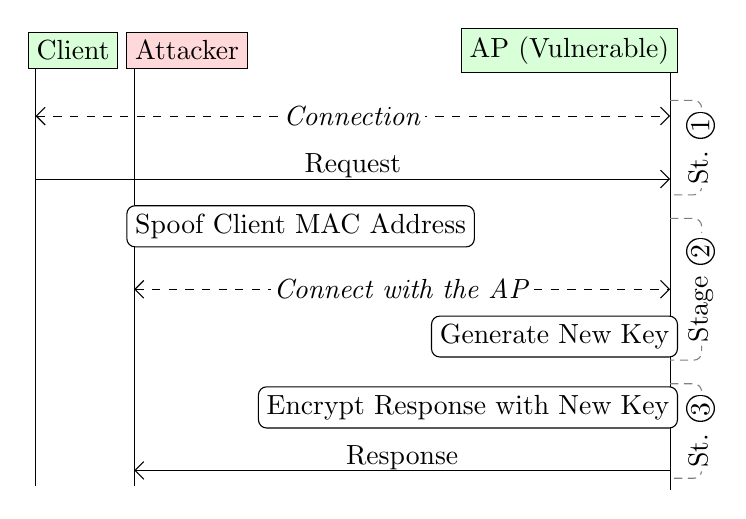
\begin{tikzpicture}
	
	% Definitions.
	\tikzstyle{every node}=[
		%font=\small,
		inner sep=3pt,
		%text height=1ex,
		%text depth=.25ex,
		%minimum height=0.40cm
	]
	\def\myarrow{Straight Barb[width=6.4pt,length=3.2pt]};
	\def\StageDepth{0.40cm};
	\def\StagePadding{0.20cm};
	\def\BubbleShiftX{0.10cm};
	\def\BubbleShiftY{0.10cm};
	
	% ---------- Header and Vertical Lines ---------
	
	\node[fill=green!15, draw] (client) {Client};
	\node[fill=red!15, draw,right=0.10cm of client.east] (attacker) {Attacker};
	\node[fill=green!15, draw,right=5.50cm of client.west] (ap) {AP (Vulnerable)};
	
	\def\TimelineShift{0.1cm}
	\coordinate (clientTop) at ([xshift=\TimelineShift]client.south west);
	\coordinate (attackerTop) at ([xshift=\TimelineShift]attacker.south west);
	\coordinate (apTop) at ([xshift=-\TimelineShift]ap.south east);
	
	\def\TimelineSize{5.30cm}
	\draw[-] (clientTop) -- ([yshift=-\TimelineSize]clientTop);
	\draw[-] (attackerTop) -- ([yshift=-\TimelineSize]attackerTop);
	\draw[-] (apTop) -- ([yshift=-\TimelineSize]apTop);
	
	% ------------ Location of Messages -----------
	
	\def\LineOffset{0.70cm}
	\def\LineOffsetContextLines{0.10cm}
	\def\LineMessageOffset{-0.10cm}
	\coordinate (line1) at ([yshift={-\LineOffset+\LineOffsetContextLines}]clientTop);
	\coordinate (line2) at ([yshift={-\LineOffset-\LineOffsetContextLines}]line1);
	\coordinate (line3) at ([yshift={-\LineOffset}]line2);
	\coordinate (line4) at ([yshift={-\LineOffset}]line3);
	\coordinate (line5) at ([yshift={-\LineOffset}]line4);
	\coordinate (line6) at ([yshift={-\LineOffset}]line5);
	\coordinate (line7) at ([yshift={-\LineOffset-2*\LineOffsetContextLines}]line6);
	
	% ================== STAGE 1 ==================
	
	% Connection.
	\draw[{\myarrow}-{\myarrow}, dashed] (line1) -- node[fill=white,draw=white,inner sep=1pt] {\emph{Connection}} (apTop |- line1);
	
	% Request.
	\draw[-{\myarrow}] (clientTop |- line2) -- node[above,yshift=\LineMessageOffset] {Request} (apTop |- line2);
	
	% Brackets for Stage.
	\draw[densely dashed, color=gray, rounded corners=0.1cm]
	([yshift=\StagePadding]line1 -| apTop) --
	([yshift=\StagePadding,xshift=\StageDepth]line1 -| apTop) -- 
	node [midway,rotate=90,color=black,fill=white,draw=white,inner sep=1pt] {St.~\circlenum{1}}
	([yshift=-\StagePadding,xshift=\StageDepth]line2 -| apTop) --
	([yshift=-\StagePadding]line2 -| apTop);
	
	% ================== STAGE 2 ==================
	
	% Re-Connection.
	\draw[{\myarrow}-{\myarrow}, dashed] (attackerTop |- line4) -- node[fill=white,draw=white,inner sep=1pt] {\emph{Connect with the AP}} (apTop |- line4);
	
	% Bubbles.
	\node[anchor=west,rounded corners=3pt,fill=white,draw] (line3node) at ([xshift=-\BubbleShiftX,yshift=\BubbleShiftY]attackerTop |- line3) {Spoof Client MAC Address};
	\node[anchor=east,rounded corners=3pt,fill=white,draw] (line5node) at ([xshift=\BubbleShiftX,yshift=\BubbleShiftY]apTop |- line5) {Generate New Key};
	
	% Brackets for Stage.
	\draw[densely dashed, color=gray, rounded corners=0.1cm]
	([yshift=\StagePadding]line3 -| apTop) --
	([yshift=\StagePadding,xshift=\StageDepth]line3 -| apTop) -- 
	node [midway,rotate=90,color=black,fill=white,draw=white,inner sep=1pt] {Stage~\circlenum{2}}
	([yshift=-\StagePadding,xshift=\StageDepth]line5 -| apTop) --
	([yshift=-\StagePadding]line5 -| apTop);
	
	% ================== STAGE 3 ==================

	% Response.
	\draw[-{\myarrow}] (apTop |- line7) -- node[above,yshift=\LineMessageOffset] {Response} (attackerTop |- line7);
	
	% Bubbles.
	\node[anchor=east,rounded corners=3pt,fill=white,draw] (line6node) at ([xshift=\BubbleShiftX,yshift=-\BubbleShiftY]apTop |- line6) {Encrypt Response with New Key};
	
	% Brackets for Stage.
	\draw[densely dashed, color=gray, rounded corners=0.1cm]
	([yshift=\StagePadding]line6 -| apTop) --
	([yshift=\StagePadding,xshift=\StageDepth]line6 -| apTop) -- 
	node [midway,rotate=90,color=black,fill=white,draw=white,inner sep=1pt] {St.~\circlenum{3}}
	([yshift=-0.5*\StagePadding,xshift=\StageDepth]line7 -| apTop) --
	([yshift=-0.5*\StagePadding]line7 -| apTop);

	\end{tikzpicture}
	\caption{Illustration of the security context overriding attack.}
	\label{fig:securitycontext:overriding}
\end{figure}


In stage~\circlenum{1} of the attack, the adversary will forward any probe requests to the \red{AP}.
If the probe requests contains an optional \red{SSID equal to TrustedNet}, then the adversary will replace TrustedNet with OtherNet, and will then forward the probe request.
Similarly, any probe responses and beacons sent by the AP will be modified by replacing OtherSSID with TrustedSSID.
As a result, the victim will think that the network TrustedSSID is nearby, even when it is not.

In stage~\circlenum{2} of the attack, the victim will attempt to connect with \red{TrustedSSID}.
The connection process starts by sending and receiving an (open) authentication frame that are forward to from and the \red{OtherAP} without modification.
Once (open) authentication completed, the client will send an association request that includes the SSID the client is connecting to.
The adversary will rewrite \red{TrustedSSID} to \red{OtherSSID} before forwarding the association request to the AP.
The association response does not contain an SSID and can therefore be forwarded to the client without modification~\mbox{\cite[Table~9-35]{ieee80211-2020}}.
After association, an 802.1X authentication handshake is performed when connecting to an enterprise \wifi{} network.
%TODO: when connecting for the first time to any protected \wifi{} network,
Finally, the \fourway{} handshake is used to negotiate fresh session keys to encrypted and authenticate data frames.
Note that these negotiated keys are dependent on the MAC addresses of the client and victim, but this does not impact the attack, because the MC-MitM allows the adversary to create a rogue clone of the AP using the same MAC address as that of \red{OtherSSID}.

\red{---TODO: Explain that authentication succeeds even though we are connecting to a different network!---}

\begin{table}
	\caption{Overview of authentication methods and whether they are vulnerable to SSID confusion attacks.}
	\begin{tabular}{lll}
	\toprule
	\red{Network} & Protocol & Affected \\
	\midrule
	Home & WEP & Yes \\
		& WPA1/2 & No \\
		%TODO: Both of these are also used for Mesh networks. So this is a bad grouping... Maybe first list SAE/802.1X and then mention the type of networks they are used in? Or not mention the type at all?
		& \red{WPA3 SAE-loop} & Yes \\
		& \red{WPA3 SAE-const} & No \\
	Enterprise & \red{802.1X} & Yes \\
	Mesh & AMPE & Yes \\
	\red{Other} & FILS & Yes \\
		& FT & Yes \\
	\bottomrule
	\end{tabular}
\end{table}

\subsection{Home Network Authentication}

\subsubsection{WEP}
% https://www.mathyvanhoef.com/2015/03/codegate-2015-goodcrypto-advanced-wep.html
The old WEP protocol is also vulnerable, \red{which is still used by 1\% of all \wifi{} networks}.

\subsubsection{WPA1/2}

\red{---Home networks are not vulnerable because the PMK is influenced by the SSID.---}

\subsubsection{WPA3}

\red{---For home networks, version~1 of WPA3 is vulnerable because the SSID never influences the PMK, but version~2 is not vulnerable because then the SSID does influence the PMK.---}

\subsection{Enterprise Network Authentication} % Enterprise networks 802.1X

\red{All Enterprise networks are vulnerable, so WPA1/2/3 is all vulnerable.
For an Enterprise network, a subsequent Fast BSS Transition would also still work, since it is not based on the SSID either.}

\subsection{Mesh Network Authentication}

\red{---TODO: With Mesh networks: ``In order to create a secure peering, mesh STAs first authenticate each other and create a mesh PMKSA. This can be done using either SAE or IEEE Std 802.1X. A mesh STA shall support SAE authentication (see 12.4). A mesh STA may support IEEE 802.1X authentication (see 4.10).''
That is followed by AMPE which does not verify the SSID.
So the attack is also possible for mesh networks it seems.---}

\subsection{Other Authentication Methods}

\subsubsection{Fast BSS Transition}

\subsubsection{FILS (Public Key)}

\subsubsection{Other}

\red{What about AP PeerKey?}

Technically also the TPK handshake for client to client communication.
But what's the point, no practical impact or realistic threat model?

% https://mrncciew.com/2023/09/25/fils-fast-initial-link-setup/
FILS Public Key authentication also looks vulnerable.
Is it realistic that two networks share the same public key?

\red{---TODO: What about the short SSID in the FILS frames?---}

\section{Attack Optimization and evaluation}
\label{sec:evaluation}

In this section we first evaluate our attack and then propose an optimized version of our attack.
Additionally, we estimate against how many enterprise users our attack is possible, and discuss the impact of channel validation on our attack.

\subsection{Evaluation}

\begin{table}
	\caption{Experiments against various clients.
	\red{Yes means that the attack indeed works against the protocols listed as vulnerable in Section~\ref{sec:attack}.
	---TODO: Is a difference between home and enterprise needed? Or infrastructure vs mesh?---}}
	\begin{tabular}{lll}
		\toprule
		& \multicolumn{2}{c}{Attack Type} \\
		\cmidrule{2-3}
		Device & Standard & Connection-Only \\
		\midrule
		Windows & \red{Yes} & \\
		iOS \\
		Android \\
		macOS \\
		\bottomrule
	\end{tabular}
\end{table}

\red{---Describe the test tool that simulates the MC-MitM to more easily test various clients. So configure Hostapd using the OtherSSID, and modify Hostapd to change this SSID to TrustedSSID in transmitted beacons, transmitted probe responses, and received association requests. That simulates a MC-MitM attack. Now check whether different clients (Linux, Windows, iOS, etc) still successfully connect.---}

Our test tool supports all major authentication methods: WEP, WPA2/3, WPA3 with SAE-Loop and SAE-Constant, PEAP, TTLS, EAP-PWD, and so on.
Additionally, test can be performed while the network is using \red{MFP} or \red{beacon protection}.

\subsection{Optimized Connection-Only Attack}

Once a client has connected, most clients no longer check the SSID in the received beacons.
This means the attacker only needs to be present while the victim is connecting to the network, and can then move the client back to the original channel.

\red{---Describe how implemented in test tool: change the SSID in the beacon only after connecting. Test several clients. Test both with and without beacon protection??---}


\subsection{Enterprise Evaluation}
\label{sec:eval:ent}

Example attack scenarios Enterprise:
\begin{itemize}
	\item Eduroam and home university \wifi{} network that use the same authentication.
	Scrape eduroam and look if the radius server is also used in other configuration guides.

	Based on scraping of the tools, we found 6 vulnerable organizations:
	eduroam.technion.ac.il
	nac.temple.edu
	radius.kuleuven.be
	radius.vse.cz
	radius.york.ac.uk
	val.ul.ie

	%TODO: \red{---TODO: Also check for public key reuse, but difference CommonName, under the assumption that the client might check the public key but not the CommonName.---} ==> This didn't immediately seem the case, so this has low priority...

	\item Telenet Wi-Free and KU Leuven university login.
	Home users can now intercept traffic!
	Confirm key is stored in AP by \red{Telenet's plaintext behavior, reply time, and disconnecting coax cable}.
	
	Also citiwifi in Luxembourg and \verb|luxfuturelab.lu| which is a similar attack (Public \wifi{} Networks).
\end{itemize}

We can test these attacks at multiple devices as well, though they have a high chance to simply work.


\subsection{Impact of Channel Validation}
\label{sec:ocv}

\red{---TODO: What about performing the attack when channel validation is enabled? Probably just do a wormhole attack or be out of range of the original AP.---}

\section{Defenses}
\label{sec:defenses}

In this section we propose, implement, and evaluate backwards-compatible defenses, and we propose updates to the 802.11 standard.

\subsection{Beacon Protection}

\subsubsection{Background}

Starting with the \red{802.11be} amendment, also called \wifi{}~7, all \red{Access Points~(APs)} must support beacon protection~\cite{ieee-mentor-mandate-beaconprot}.
When beacon protection is used, the AP will authenticate all transmitted beacons using a symmetric key.
Clients obtain this symmetric key in the \fourway{} handshake when connecting to the network.

When using beacon protection, an adversary is no longer able to change the SSID included in beacons \red{after the client has connected} (see stage~\circlenum{3} in Figure~\ref{fig:ssidconfusion}).
This implies that an adversary would, in theory, be able to detect the SSID confusion attack \emph{after} being connected to the network.

\subsubsection{Experiments}

\red{---Can we still perform the attack when beacon protection is being used? Probably yes, because the beacons only get verified once connected, at least by wpa\_supplicant.---}
%Doesn't look like it on Linux, see mac80211/mlme.c.

%TODO: We won't actually request this CVE...
\red{This vulnerability in} \verb|wpa_supplicant| \red{was assigned CVE-2023-XXXXXXX}.

\subsubsection{Verification of pre-auth beacon}

Normally a reference beacon should be saved, which is then checked once connected~\cite{vanhoef-wisec2020}.
This is currently not done by Linux.

\red{Demonstrate that the attack is prevented in all cases when the AP and client use beacon protection, with reference beacon comparison, and optionally with SSID checking in received beacons.}

Older networks will use a hidden SSID and in that case beacon protection cannot be used to prevent the attack.
But enabling beacon protection AND advertising the SSID will prevent the attack, since the victim will then either get the real beacon with SSID or will be unable to verify a forged beacon.

\subsection{Other Defenses}

Backwards-compatible:
\begin{itemize}
	\item Use a different RADIUS server for each network.
	For home networks, use a different password for each different SSID.
	%\item Use a different inner/outer identity for each network? Depends on whether the RADIUS server knows the network the request came from.
	\item Modify the client OS to include a flag whether the authenticity of the SSID is currently verified.
	Alternatively, instead of giving access to the SSID, the OS could make available the CommonName used in enterprise networks.
\end{itemize}

Protocol changes:
\begin{itemize}
	\item The 4-way handshake itself could (again) include the SSID.
\end{itemize}


\section{Related Work}
\label{sec:relatedwork}

Cassola et al.\ attacked enterprise WPA2 networks by creating a rogue clone of the network, where the SSID of the rogue clone included extra invisible characters~\cite{cassola2013practical}.

\red{Some kind of Apple continuity bug where the victim can be tricked into connecting to any SSID~\cite{stute2021disrupting}.}

\red{The Tryst protocol proposed by Greenstein et al, which has as purpose to prevent user tracking, would also prevent our attack~\cite{greenstein2008improving}.
Unfortunately, this protocol is not adopted in practice, and requires the client and AP to store additional state after the first connection.}

\section{Conclusion}
\label{sec:conclusion}

We highlighted that users, or their apps, make security-sensitive decisions based on the \red{SSID} they are connected to.
For instance, a VPN can automatically get disabled when connected to a trusted SSID. 
However, we demonstrated that the SSID can be \red{spoofed} by an adversary, even when enterprise \red{encryption} or home WPA3 \red{encryption} is used.
\red{This is caused by a design flaw in the IEEE 802.11 standard and it was assigned CVE-2023-XXXXXXX}.

A backwards-compatible defense is to use beacon protection and verifying the authenticity of \red{a reference beacon} before exchanging data frames.
Alternatively, the 802.11 standard can be updated to authenticate the \red{SSID} of a network during the \fourway{} handshake.

%\vspace{-0.05cm}
\begin{acks}
This research is partially funded by the Research Fund KU Leuven, and by the Flemish Research Programme Cybersecurity.
\end{acks}

%\vspace{-0.05cm}
\bibliographystyle{ACM-Reference-Format}
\bibliography{references}

% \appendix
% \section{Research Methods}
% \subsection{Part One}

\end{document}
\endinput